\newpage

\section{Introduction}\label{introduction}

Ce rapport présente le développement d'une application multisupport de
moteurs de recherche de documents dans une bibliothèque de livres au
format textuel. OpenYourMind est une application web et mobile qui se
distingue par sa capacité à interagir avec l'utilisateur, offrant des
fonctionnalités dynamiques et réactives. Ce projet met l'accent sur deux
aspects essentiels : la pertinence et la performance du moteur de
recherche. La pertinence est évaluée à l'aide de tests utilisateurs,
tandis que la performance est mesurée à travers les temps de réponse du
moteur de recherche.

\section{Choix Technologique}\label{choix-technologique}

Pour développer notre application, nous avons opté pour Flutter pour le
développement de l'interface utilisateur et Django pour le backend afin
de créer une plateforme robuste, performante et conviviale. En
choisissant Flutter, nous bénéficions d'un framework cross-platform
permettant une conception fluide pour les utilisateurs iOS, Android et
web. De plus, ce langage offre une bibliothèque de widgets
personnalisables très riche, ce qui rend le développement Front-end
beaucoup plus simple. Concernant le Backend, nous avons choisi Django
puisqu'il simplifie l'interaction avec la base de données grâce à son
mapping d'objet relationnel. En outre, étant basé sur Python, Django
offre une flexibilité pour intégrer des bibliothèques, telles que celles
pour le traitement de chaînes de caractères et des graphes, facilitant
ainsi le développement des fonctionnalités clés de notre moteur de
recherche.

\section{Setup}\label{setup}

Afin de tester notre motteur de recherche il est necessaire d'effecutuer
les installations decrites dans cette section.

\subsection{Installation}\label{installation}

\subsubsection{Backend}\label{backend}

\begin{itemize}
\tightlist
\item
  Python \textgreater= 3.12

  \begin{itemize}
  \tightlist
  \item
    \href{https://www.djangoproject.com/}{Django}
  \item
    \href{https://www.nltk.org/}{Nltk}
  \item
    \href{https://networkx.org/}{Networkx}
  \item
    \href{https://docs.python-requests.org/en/master/}{Requests}
  \end{itemize}
\end{itemize}

\begin{Shaded}
\begin{Highlighting}[]
\ExtensionTok{pip}\NormalTok{ install django djangorestframework nltk requests networkx}
\end{Highlighting}
\end{Shaded}

\subsubsection{Construction de la base de
données}\label{construction-de-la-base-de-donnuxe9es}

La base de données n'est pas incluse dans le rendu. Vous devez la
construire vous-même, cela prend BEAUCOUP DE TEMPS ET DE RESSOURCES.

\begin{Shaded}
\begin{Highlighting}[]
\BuiltInTok{cd}\NormalTok{ backend}
\ExtensionTok{python}\NormalTok{ manage.py makemigrations}
\ExtensionTok{python}\NormalTok{ manage.py migrate}
\ExtensionTok{python}\NormalTok{ manage.py scrape\_books}
\ExtensionTok{python}\NormalTok{ manage.py create\_indexTable}
\ExtensionTok{python}\NormalTok{ manage.py create\_metadata}
\end{Highlighting}
\end{Shaded}

\subsubsection{Frontend}\label{frontend}

\begin{itemize}
\tightlist
\item
  \href{https://flutter.dev/}{Flutter}
\end{itemize}

Pour installer \href{https://flutter.dev/}{Flutter}, voir la
\href{https://flutter.dev/docs/get-started/install}{documentation
officielle}.

\subsection{Démarrage}\label{duxe9marrage}

\subsubsection{Backend}\label{backend-1}

Pour démarrer le serveur, exécuter la commande suivante~:

\begin{Shaded}
\begin{Highlighting}[]
\BuiltInTok{cd}\NormalTok{ backend}
\ExtensionTok{python}\NormalTok{ manage.py runserver}
\end{Highlighting}
\end{Shaded}

\subsubsection{Frontend}\label{frontend-1}

Pour démarrer l'application frontend, exécuter la commande suivante~:

\begin{Shaded}
\begin{Highlighting}[]
\BuiltInTok{cd}\NormalTok{ frontend}
\ExtensionTok{flutter}\NormalTok{ pub get}
\ExtensionTok{flutter}\NormalTok{ run}
\end{Highlighting}
\end{Shaded}

Puis choisissez l'appareil sur lequel vous souhaitez exécuter
l'application.

\section{Backend}\label{backend-2}

\subsection{Architecture}\label{architecture}

Le back est basé sur le framework Django, qui est un framework web
Python de haut niveau qui encourage un développement rapide et une
conception propre et pragmatique. \newpage

\begin{itemize}
\tightlist
\item
  \texttt{backend/gutendex/}

  \begin{itemize}
  \tightlist
  \item
    \texttt{management/commands/} : Commandes personnalisées pour la
    gestion de la base de données.

    \begin{itemize}
    \tightlist
    \item
      \texttt{create\_indexTable.py} : Création de la table d'index
      inversé.
    \item
      \texttt{create\_metadata.py} : Création des métadonnées des
      livres, utilisées pour l'affichage des résultats de recherche, le
      filtrage et le tri.
    \item
      \texttt{scrape\_books.py} : Récupération des 1660 premiers à
      partir de l'API de \href{https://www.gutenberg.org/}{Gutenberg}.
    \end{itemize}
  \item
    \texttt{models.py} : Définition des modèles de données.
  \end{itemize}
\end{itemize}

\subsubsection{Base de données}\label{base-de-donnuxe9es}

Au vu de la taille du projet, nous avons opté pour une architecture
simple de type monolithique, car elle est plus facile à gérer et à
déployer. Cependant, nous avons pris soin de séparer les partis métiers
et les parties de gestion de la base de données.

\textbf{Scraping (Farouck Cherfi) : }

\newpage

Voici à titre indicatif, un diagramme de la base de données :

\begin{figure}
\centering
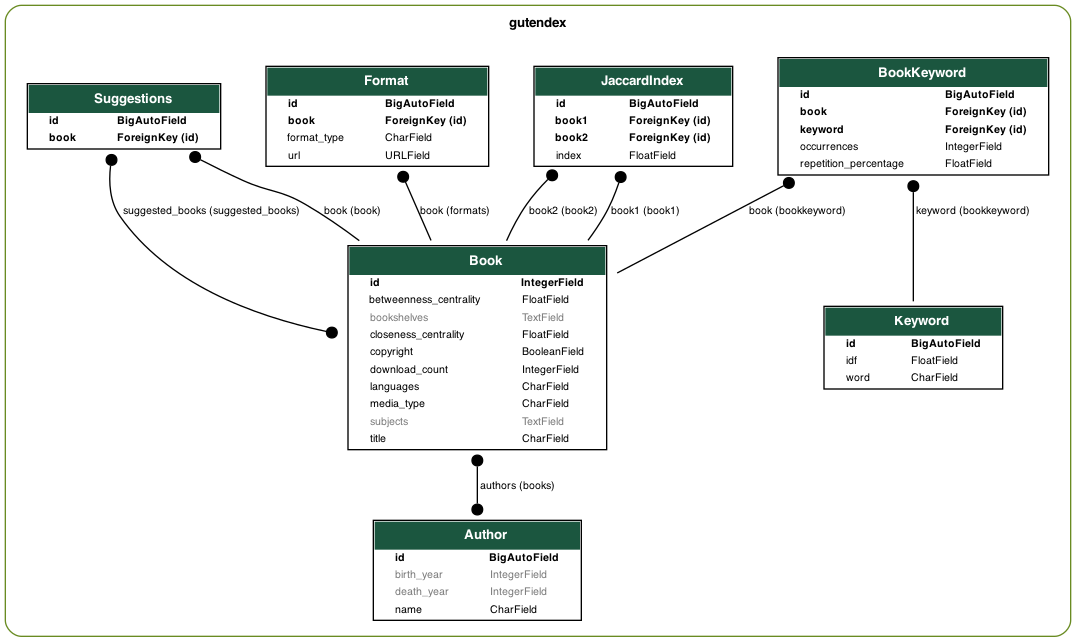
\includegraphics{../backend/db.png}
\caption{Database Diagram}
\end{figure}

\subsubsection{EndPoints}\label{endpoints}

\begin{itemize}
\tightlist
\item
  \texttt{top-books/} : Récupération des livres les plus téléchargés.
\item
  \texttt{search/\textless{}sentence\ or\ regex\textgreater{}/} :
  Recherche de livres par phrase.
\item
  \texttt{book/\textless{}bookid\textgreater{}/} : Récupération d'un
  livre par son identifiant.
\item
  \texttt{suggest/\textless{}bookid\textgreater{}/} : Suggestions de
  recherche.
\end{itemize}

\subsection{Recherche}\label{recherche}

\begin{itemize}
\tightlist
\item
  \texttt{backend/gutendex/helpers.py} : Fonctions de recherche.
\end{itemize}

Le moteur de recherche est basé sur l'indexation inversée des livres.
Une fois nos livres compatibles avec les mots clés récupérés, il est
important de les classer par pertinence.

\subsubsection{Heuristiques}\label{heuristiques}

Pour notre heuristique de classements, nous avons utilisé 3 valeurs :

\begin{itemize}
\tightlist
\item
  \textbf{AVERAGE TF-IDF} : Term Frequency-Inverse Document Frequency
  est une mesure statistique utilisée pour évaluer l'importance d'un mot
  dans un document par rapport à une collection de documents ici on
  utilise une version modifiée afin de prendre en compte un ensemble de
  mots clés.
\end{itemize}

Voici la formule utilisée pour calculer le TF d'un terme pour un
document:
\[TF(t) = \frac{\text{Nombre de fois où le terme apparaît dans le document}}{\text{Nombre total de termes dans le document}}\]
Voici la formule utilisée pour calculer l'IDF d'un terme:
\[IDF(t) = \log\left(\frac{\text{Nombre total de documents}}{\text{Nombre de documents contenant le terme}}\right)\]

\begin{itemize}
\item
  \textbf{Betweenness Centrality} : Elle mesure le nombre de fois qu'un
  nœud est sur le chemin le plus court entre deux autres nœuds.
\item
  \textbf{Closseness Centrality} : Elle mesure la distance moyenne entre
  un nœud et tous les autres nœuds.
\end{itemize}

Les deux dernières valeurs étant basées sur des graphes, voici sa
construction :

Soit \(G = (V, E)\) un graphe géométrique où \(V\) est l'ensemble des
livres et \(E\) l'ensemble des arêtes.

On construit \(E\) de la manière suivante :

\begin{itemize}
\tightlist
\item
  On determine la moyenne des similarités de Jaccard entre chaque livre
  \[ k = \frac{\sum{v,u \in V*V} \text{Jaccard}(u, v)}{|V|*|V|-1}\ u \neq v\]
\item
  Pour éviter de se connecter a trop de livres, on augemente \(k\) de
  30\%. \[ threashold = k + 0.3k\]
  \[ E = \{(u, v) \in V \times V \mid \text{Jaccard}(u, v) \geq threashold\}\]
\end{itemize}

Une fois ses valeurs calculées, on les combine pour obtenir un score de
pertinence d'un livre par rapport à un ensemble de mots clés

\[Score(Keywords, Book) = 0.7*\text{AVG-TF-IDF}(Keywords, Book)\]
\[ +\ 0.15*\text{Betweenness}(Book) + 0.15*\text{Closeness}(Book)\]

\subsection{Suggestions}\label{suggestions}

Dans le but d'améliorer l'expérience utilisateur, nous avons implémenté
un système de suggestions de recherche. Ce système est basé sur la
recherche de livres similaires à celui sélectionné par l'utilisateur.

Nous avons utilisé essayer deux approches pour déterminer la similarité
entre les livres :

\subsubsection{Similarité par le
titre}\label{similarituxe9-par-le-titre}

Ici, l'approche est basée sur le titre du livre. La méthode est la
suivante :

\begin{enumerate}
\def\labelenumi{\arabic{enumi}.}
\tightlist
\item
  On récupère les mots clés du titre.
\item
  On relance une recherche avec les deux mots clés ayant le plus grand
  IDF.
\item
  On retourne les résultats.
\end{enumerate}

\subsubsection{Similarité par le
contenu}\label{similarituxe9-par-le-contenu}

Ici l'approche place plus d'emphase sur le contenu, La méthode est la
suivante, on récupère simplement les livres connectés sur le graphe
décrit \hyperref[heuristiques]{précédemment}.

\subsubsection{Comparaison}\label{comparaison}

Nous avons choisi après plusieurs tests d'éliminer la première méthode,
car dans les cas où le titre contient des mots très courants, la
recherche n'est pas pertinente. Un exemple de titre non pertinent est
``Le Rouge et le Noir'', les mots clés Rouge/Noir ne permettent pas de
déterminer des informations sur le contenu du livre et donc notre
\hyperref[heuristiques]{AVG-TF-IDF} n'est pas pertinent, invalidant la
méthode de scoring.

\subsection{Performance}\label{performance}

Dans cette section, nous allons discuter de la performance de notre
moteur de recherche. Nous avions un objectif principal :

\begin{itemize}
\tightlist
\item
  Réduire le temps de réponse du moteur de recherche
\end{itemize}

Pour ce faire, nous avons utilisé une technique principale le précalcul,
ainsi nous avons precalculé les valeurs de
\hyperref[heuristiques]{Betweenness},
\hyperref[heuristiques]{Closeness}, \hyperref[heuristiques]{TF-IDF} pour
chaque livre et chaque mot clé.

\subsubsection{Tests}\label{tests}

Nous avons testé la performance de notre moteur de recherche sur un
ensemble de 140 requêtes de type keyword/regex aléatoire. Voici les
résultats de nos tests :

\begin{figure}
\centering
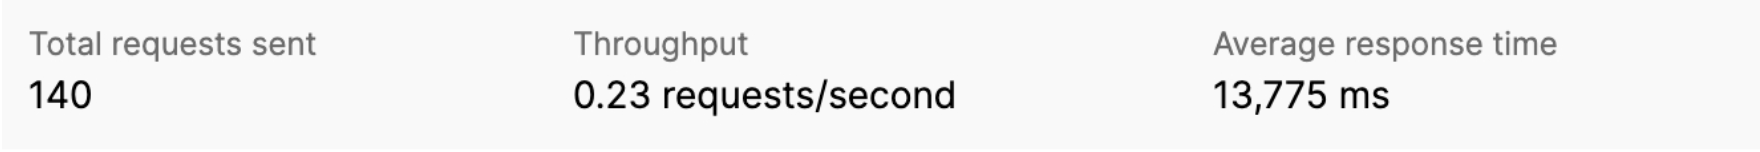
\includegraphics{./avgTotal.png}
\caption{Average Response Time}
\end{figure}

\begin{figure}
\centering
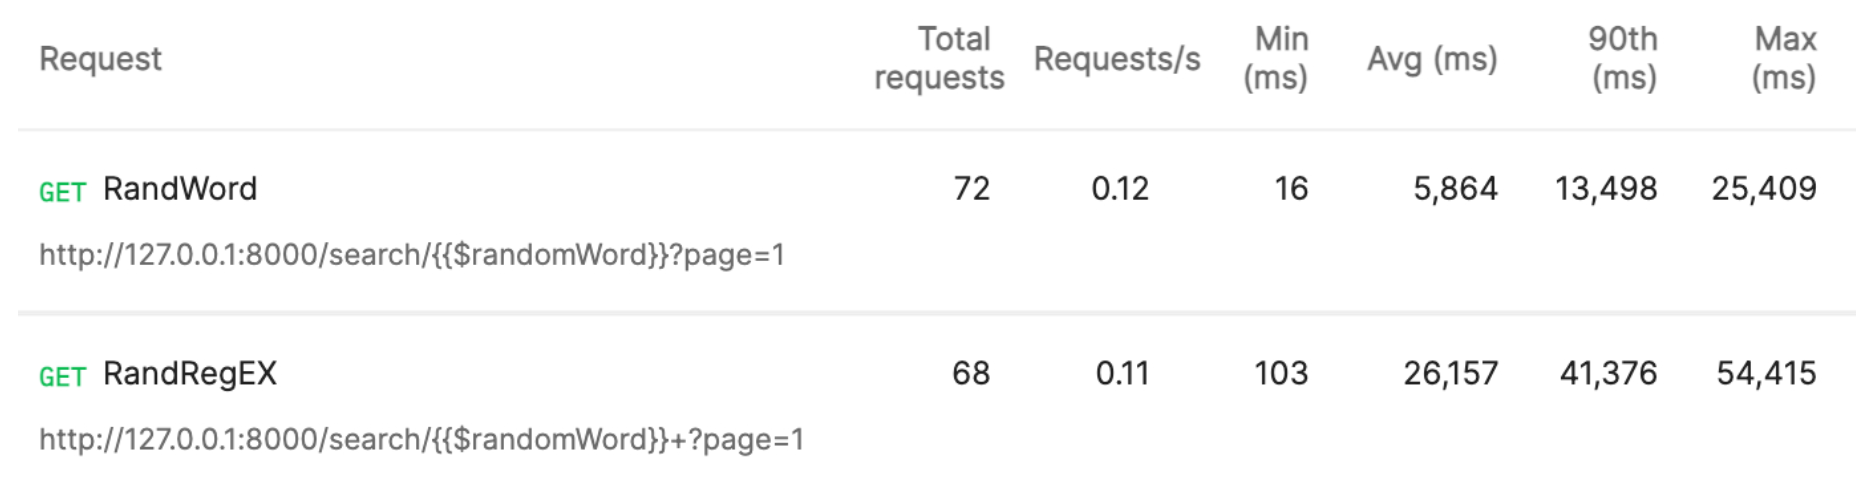
\includegraphics{./avgPerEndPoint.png}
\caption{Per Endpoint Response Time}
\end{figure}

\section{Frontend}\label{frontend-2}

\subsection{Architecture}\label{architecture-1}

Pour le FrontEnd, nous avons choisi de baser notre architecture sur le
concept de séparation des préoccupations en organisant ainsi nos fihier
selon leurs roles qui gerent un aspect precis de notre application.

\begin{itemize}
\tightlist
\item
  \texttt{/frontend/lib}

  \begin{itemize}
  \tightlist
  \item
    \texttt{main.dart} : Ce fichier constitue le point d'entrée de notre
    application.
  \item
    \texttt{routes.dart} : Le fichier responsable de la gestion des
    routes de navigation au sein de l'application.
  \item
    \texttt{theme.dart} : La gestion des aspects visuels et des styles
    de notre application se fait dans ce fichier.
  \item
    \texttt{views} : Le dossier où on stocke les différents écrans/pages
    de votre application.
  \item
    \texttt{components} : Répertoire des composants réutilisables de
    notre application.
  \item
    \texttt{apis}

    \begin{itemize}
    \tightlist
    \item
      \texttt{apis/ApiCall.dart} : Ce fichier dans le dossier apis
      contient des fonctions pour effectuer des appels API vers le
      backend ou d'autres services externes.
    \end{itemize}
  \item
    \texttt{manager}

    \begin{itemize}
    \tightlist
    \item
      \texttt{manager/book\_manager.dart} : La gestion de la logique
      métier se fait dans le dossier manager, plus précisément dans le
      fichier book\_manager.dart, où l'on trouve les différentes
      opérations liées aux livres.
    \end{itemize}
  \item
    \texttt{models}

    \begin{itemize}
    \tightlist
    \item
      \texttt{models/book.dart} : Il s'agit du modèle de données pour
      représenter les informations sur les livres..
    \end{itemize}
  \end{itemize}
\end{itemize}

\subsection{Vues}\label{vues}

Notre Application se compose pricipalement de 3 vues ``Home'',
``result\_page'' et ``book\_description\_page''.

\subsubsection{Home}\label{home}

Pour la page d'accueil, nous avons opté pour un design simple et
intuitif en intégrant notre composant app\_bar\_Custom et en plaçant au
centre de la page notre barre de recherche, juste au-dessus de la
section affichant les 10 meilleurs livres qui utilise le composant
multiple\_book qu'on detaillera par la suite. Lorsque la page est
initialisée, la méthode initState() est appelée, chargée de récupérer
les meilleurs livres à afficher en invoquant la méthode \_loadTopBooks()
du BookManager.

Cette méthode effectue une requête asynchrone pour obtenir les meilleurs
livres à partir du backend. Une fois les données chargées, l'état de la
page est mis à jour avec les livres récupérés en utilisant setState().
De plus, selon l'état de la variable books, une barre de progression
circulaire est affichée pendant le chargement des données.

\subsubsection{Page resultat}\label{page-resultat}

La page resultat est un widget qui prend en paramètre search, le terme
de recherche saisi par l'utilisateur. Lorsque la page est initialisée
(initState()), la méthode \_loadResultBooks() est appelée pour charger
les résultats de recherche pour la première page. La classe contient
également une méthode \_loadResultAndUpdateBooks() qui est appelée pour
charger et mettre à jour les résultats de recherche. La méthode
\_searchAndUpdateBooks() est appelée lorsqu'une nouvelle recherche est
effectuée dans la page resultat. Elle réinitialise les résultats de
recherche actuels, met à jour le terme de recherche actuel et charge les
nouveaux résultats de recherche.

Visuellement La page se compose d'ne AppBar personnalisée (AppBarCustom)
mais qui contient une barre de recherche cette fois. Le corps de la page
contient soit un indicateur de progression circulaire si les résultats
de recherche sont en cours de chargement, soit la liste des résultats de
recherche organisé avec une grille dans le composant multiple\_book.Des
boutons de navigation entre les pages sont également inclus pour
permettre à l'utilisateur de passer aux résultats suivants ou
précédents.

Le système de pagination mis en œuvre dans la classe ResultPage repose
sur une gestion dynamique de l'état de la page courante (currentPage) et
du terme de recherche actuel (currentSearch).l'état des boutons est
ajusté en fonction de la disponibilité des résultats pour les pages
correspondantes par exemple, si l'utilisateur se trouve sur la première
page de résultats, le bouton ``page précédente'' est désactivé car il
n'y a pas de page précédente à afficher. Lorsqu'un bouton est cliqué, la
valeur de currentPage est mise à jour et les résultats de la nouvelle
page sont chargés via une requête asynchrone, mettant à jour l'affichage
des résultats.

\subsubsection{Page Book Description}\label{page-book-description}

Cette vue contient plusieurs éléments visuels pour présenter les détails
d'un livre sélectionné : une image du livre, une carte affichant les
informations détaillées du livre (les auteurs , la categorie ..), et un
bouton qui ouvre un onglet dans le navigateur permettant à l'utilisateur
d'acceder au lien qui contient le texte et de lire le livre. En dessous
de ces details, des livres suggérés sont disponibles, ils sont affichés
sous forme de liste à l'utilisateur en utisant encore une fois notre
composant multiple\_book.

Lorsque la page est chargée, elle récupère une liste de livres suggérés
basée sur le livre sélectionné à l'aide de la méthode
\_loadSuggestedBooks(). Cette méthode utilise une requête asynchrone
pour obtenir les livres suggérés à partir du backend

\subsection{Composants}\label{composants}

Comme mentionné précédemment, pour garantir la réutilisabilité de notre
code, nous avons développé plusieurs composants dans notre application.
Ces composants sont appelés à partir de différentes vues pour assurer
une cohérence visuelle. Voici une brève description des composants les
plus importants :

\subsubsection{App Bar}\label{app-bar}

L'app bar est un element qui est present dans toutes les vues de notre
application. Il permet d'afficher une app bar personnalisée avec la
possibilité d'inclure une barre de recherche. Le composant prend en
compte plusieurs attributs pour configurer son comportement :

\begin{itemize}
\tightlist
\item
  search: permet de spécifier le terme de recherche actuel.
\item
  isSearchBar: indique si la barre de recherche doit être affichée.
\item
  onSearch: définit une fonction de rappel appelée lorsqu'une recherche
  est soumise.
\item
  isReset: contrôle la réinitialisation du composant lors de sa
  fermeture.
\end{itemize}

Visuellement le composant génère l'app bar en fonction de ces attributs
: s'il faut afficher une barre de recherche, celle-ci est intégrée avec
éventuellement un bouton de retour en arrière ; sinon, seul le logo de
l'application est affiché au centre.

\subsubsection{La barre de recherche}\label{la-barre-de-recherche}

On ne peut certainement pas parlet d'un moteur de recherche sans le
composant barre de recherche. Dans notre application, Cet element est
conçu pour être flexible et adaptable qui peut être intégré dans l'app
bar ou utilisée de manière autonome dans d'autres pages. Ce composant
prend en compte plusieurs attributs pour ajuster son comportement :

\begin{itemize}
\tightlist
\item
  search: qui représente le terme de recherche actuel, s'il y en a un.
\item
  isAppbar: un booléen indiquant si la barre de recherche est intégrée
  dans l'app bar.
\item
  onSearch: une fonction de rappel appelée lorsqu'une recherche est
  soumise.
\end{itemize}

Visuellement, on utilise un TextField, qui est configuré avec des
options de style et de comportement en fonction des attributs spécifiés.
L'apparence de la barre de recherche varie en fonction de la présence ou
de l'absence d'une app bar, ainsi que de la valeur du texte saisi.

\subsubsection{Multiple Book}\label{multiple-book}

Le composant multiple\_Book est conçu pour présenter une liste de livres
dans Notre application. Il est egalement adaptable et peut pouvant
utilisé tant pour afficher les résultats d'une recherche de livres que
pour mettre en avant une sélection recommandée, suivant le contexte de
l'application. Le widget prend ainsi en compte plusieurs attributs :

\begin{itemize}
\tightlist
\item
  isResultPage : un booléen indiquant si le widget est utilisé dans une
  page de résultats de recherche.
\item
  books : une liste de livres à afficher.
\item
  label : une chaîne de caractères représentant un libellé associé à la
  liste de livres, comme ``Résultats de recherche'' ou ``Livres
  recommandés''.
\end{itemize}

L'élement comprend un en-tête texte exposant le libellé spécifié, suivi
d'une liste disposée horizontalement ou d'une grille verticale de
livres, selon le contexte de l'application. Chaque livre est représenté
par le composant Single\_book, permettant une présentation détaillée de
ses informations.

\subsection{Gestion cross-platform}\label{gestion-cross-platform}

Les composants de notre interface utilisateur sont conçus de manière à
s'adapter de manière dynamique aux différentes tailles d'écran, offrant
ainsi une experience agreable pour les utilisateurs web ou mobile. Cette
adaptation est réalisée en utilisant des fonctionnalités telles que
MediaQuery pour obtenir les dimensions de l'écran et ajuster les
éléments en conséquence. Par exemple, dans le widget MultipleBook, la
disposition des livres est adaptée en fonction de la taille de l'écran :
une disposition en grille est privilégiée sur les écrans larges pour
optimiser l'utilisation de l'espace, tandis qu'une liste verticale est
préférée sur les écrans plus étroits pour faciliter la navigation et la
lisibilité. Ce processus d'adaptation permet d'offrir une expérience
utilisateur optimale, quel que soit le périphérique utilisé pour accéder
à l'application.

\newpage

\section{Conclusion}\label{conclusion}

En conclusion, le projet OpenYourMind est basé sur une conception
centrée sur l'utilisateur pour créer un moteur de recherche de
bibliothèque efficace et convivial. En utilisant les technologies
Flutter et Django, nous avons pu exploiter les avantages de chaque
technologie pour offrir une expérience utilisateur cohérente et réactive
sur une variété de plateformes. L'utilisation de composants
réutilisables, une architecture bien pensée et une attention
particulière portée à la performance et à la pertinence du moteur de
recherche ont permis de créer une application robuste et performante.
